%!TEX TS-program = xelatex
%!TEX encoding = UTF-8 Unicode
%!BIB TS-program = bibtex
%!TeX spellcheck = en_US
\documentclass[12pt]{article}
\usepackage[english]{babel}
\usepackage{url}
\usepackage[utf8x]{inputenc}
\usepackage{amsmath}
\usepackage{graphicx}
\graphicspath{{images/}}
\usepackage{parskip}
\usepackage{fancyhdr}
\usepackage{vmargin}
\usepackage{enumerate}
\usepackage[T1]{fontenc}
\usepackage{newpxtext,newpxmath}
\usepackage{booktabs}
\usepackage{siunitx}
\usepackage[version=4]{mhchem}
\usepackage{hyperref}
\usepackage{bm}
\usepackage{breqn}
\setmarginsrb{3 cm}{2.5 cm}{3 cm}{2.5 cm}{1 cm}{1.5 cm}{1 cm}{1.5 cm}
\sisetup{inter-unit-product = \ensuremath{{}\cdot{}}}
\DeclareTextCommand{\nobreakspace}{T1}{\leavevmode\nobreak\ }
\newcommand{\ii}{{\mathrm{i}}}
\newcommand{\ee}{\mathrm{e}}

\title{Solid State Physics HW 2}								% Title
\author{XYZ}								% Author
\date{}											% Date

\makeatletter
\let\thetitle\@title
\let\theauthor\@author
\let\thedate\@date
\makeatother

\pagestyle{fancy}
\fancyhf{}
\rhead{\theauthor}
\lhead{\thetitle}
\cfoot{\thepage}

\newcommand*{\rmn}[1]{\romannumeral#1}
\newcommand*{\RMN}[1]{\uppercase\expandafter{\romannumeral#1}}
\begin{document}

%%%%%%%%%%%%%%%%%%%%%%%%%%%%%%%%%%%%%%%%%%%%%%%%%%%%%%%%%%%%%%%%%%%%%%%%%%%%%%%%%%%%%%%%%

\begin{titlepage}
	\centering
	\vspace*{0.5 cm}
	
\includegraphics[scale = 0.25]{NewEngineeringDkBlue.png}\\[1.0 cm]	% University Logo
	\textsc{\Large Applied Physics and Applied Mathematics\\
		\large with Materials Science and Engineering}\\[2.0 cm]	% University Name
	\textsc{\Large APPH 6081}\\[0.5 cm]				% Course Code
	\rule{\linewidth}{0.2 mm} \\[0.4 cm]
	{ \huge \bfseries \thetitle}\\
	\rule{\linewidth}{0.2 mm} \\[1.5 cm]

	\begin{minipage}{0.4\textwidth}
		\begin{flushleft} \large
			\emph{Submitted To:}\\
			Chris Marianetti\\
			Assoc. Professor\\
			APAM Department\\
		\end{flushleft}
	\end{minipage}~
	\begin{minipage}{0.4\textwidth}

		\begin{flushright} \large
			\emph{Submitted By :} \\
			XYZ\\
			\texttt{xyz}\\
			Fall 2016\\
		\end{flushright}

	\end{minipage}\\[2 cm]


\end{titlepage}

\section*{Problem \RMN{1}}
\begin{enumerate}[(a)]
	\item In the well, we have $V(x) = 0$, thus
	      Schr\"{o}dinger equation will be written as:
	      \begin{equation}
	      	-\frac{\hbar^2}{2m}\dfrac{\partial^2 \psi(x)}{\partial x^2} = E\psi(x),
	      \end{equation}
	      so $\psi(x) = C_1 \cos\big(\sqrt{\lambda}x\big) + C_2 \sin\big(\sqrt{\lambda}x\big)$, where $\lambda=\frac{2mE}{\hbar^2}$.

	      Boundary condition:
	      \begin{align}
	      	\psi(0) & = C_1 = 0                                                                                  \\
	      	\psi(L) & = C_1 \cos\big(\sqrt{\lambda}L\big) + C_2 \sin\big(\sqrt{\lambda}L\big) = 0\label{eq:psiL}
	      \end{align}
	      For \eqref{eq:psiL}, we have $\sin\big(\sqrt{\lambda}L\big) = 0$, thus $\sqrt{\lambda}L = \frac{n\pi}{L} \Rightarrow \lambda_n = \big(\frac{n\pi}{L}\big)^2$ where $n= 1, 2, 3,\ldots$
	      And based on orthonormal property,
	      \begin{equation}
	      	\int_0^L \psi^\ast(x)\psi(x) \, dx = \int_0^L C_2^2 \sin^2\big(\sqrt{\lambda}x\big) = 1,
	      \end{equation}
	      therefore $C_2 = \sqrt{\frac{2}{L}}$.
	      So
	      \begin{equation}
	      	\psi_n(x) =  \sqrt{\frac{2}{L}} \sin\bigg(\frac{n\pi}{L}x\bigg)
	      \end{equation}
	      where $n=  1,  2,  3\ldots$ are eigenfunctions, the corresponding eigenvalues are $\lambda_n = \big(\frac{n\pi}{L}\big)^2$.
	      The smallest eigenvalue is called zero-point energy, $\frac{\hbar^2\pi^2}{2m L^2}$.
	      DOS is defined as
	      \begin{equation}
	      	g(E) = \frac{1}{V}\frac{dZ}{dE},
	      \end{equation}
	      where $Z$ is the number of one-electron levels,
	      so it can be written as
	      \begin{equation}
	      	g(E) = \frac{1}{\hbar\pi}\sqrt{\frac{m}{2E}}.
	      \end{equation}
	\item Boundary conditions are
	      \begin{align}
	      	\psi(x+ L) & = \psi(x),  \\
	      	\psi'(x+L) & = \psi'(x).
	      \end{align}
	      Substitute into $\psi(x) = C_1 \cos\big(\sqrt{\lambda}x\big) + C_2 \sin\big(\sqrt{\lambda}x\big)$, where $\lambda=\big(\frac{2mE}{\hbar^2}\big)^2$, we have
	      \begin{multline}
	      	C_1 (\cos\big(\sqrt{\lambda}x\big)\cos(\sqrt{\lambda} L) - \sin\big(\sqrt{\lambda}x\big)\sin\big(\sqrt{\lambda}L\big)) \\+ C_2 (\sin\big(\sqrt{\lambda}x\big)\cos\big(\sqrt{\lambda}L\big) + \cos\big(\sqrt{\lambda}x\big)\sin\big(\sqrt{\lambda}L\big))\\ =
	      	C_1 \cos\big(\sqrt{\lambda}x\big) + C_2 \sin\big(\sqrt{\lambda}x\big),
	      \end{multline}
	      \begin{multline}
	      	-C_1 (\sin\big(\sqrt{\lambda}x\big)\cos\big(\sqrt{\lambda}L\big) +
	      	\cos\big(\sqrt{\lambda}x\big)\sin\big(\sqrt{\lambda}L\big))\\
	      	+C_2 (\cos\big(\sqrt{\lambda}x\big)\cos\big(\sqrt{\lambda}L\big) -
	      	\sin\big(\sqrt{\lambda}x\big)\sin\big(\sqrt{\lambda}L\big)
	      	)\\
	      	= -C_1 \sin\big(\sqrt{\lambda}x\big) + C_2 \cos\big(\sqrt{\lambda}x\big).
	      \end{multline}
	      The simplest way to solve these equations is to set
	      \begin{equation}
	      	\sqrt{\lambda}(x+L) = \sqrt{\lambda}x + \sqrt{\lambda}L = \sqrt{\lambda}x + 2k\pi,
	      \end{equation}
	      therefore $\sqrt{\lambda}L = 2k\pi$, so $\lambda = \big(\frac{2k\pi}{L}\big)^2$.
	      Thus eigenvalues is
	      \begin{equation}
	      	E = \frac{2\hbar^2k^2\pi^2}{mL^2}.
	      \end{equation}
	      Eigenfunctions are $\psi_k = \cos \big(\frac{2k\pi}{L}x\big)$ and $\psi_k = \sin \big(\frac{2k\pi}{L}x\big)$.
	      DOS is
	      \begin{equation}
	      	g(E) = \frac{1}{\hbar\pi}\sqrt{\frac{m}{8E}}.
	      \end{equation}
	\item The energy difference is $4$ times. Consider $L$ is infinite, then in Qu.\! 1(a) the wave transfers through $[0, \infty)$, and in Qu.\! 1(b) the wave transfers through $(-\infty, \infty)$, so the second wavelength is a half of the first. According to de Broglie relation, $k = \frac{2\pi}{\lambda}$, so the second wave vector twice as the first. And for free particle,
	      $E= \frac{\hbar^2k^2}{2m}$, so the second eigenvalue, i.e.\ , is $4$ times as the first. In short, this is because 1(a) is standing wave and 1(b) is propagating wave.
	      %        Here is another perspective to view this problem. For a free 1D particle, its DOS is
	      %        \begin{equation}
	      %                g(E) = \bigg(\dfrac{2m}{\hbar^2\pi^2}\bigg)^{1/2} E^{-1/2},
	      %        \end{equation}
\end{enumerate}


\section*{Problem \RMN{2}}
We have
\begin{equation}
	k_F^3 = 3 \pi^2 n,
\end{equation}
where
\begin{equation}
	n = \frac{\rho N_A}{M},
\end{equation}
here $M$ denotes Molar mass, $N_A$ is Avogadro constant.

Then $\varepsilon_F = \frac{\hbar^2 k_F^2}{2m}$ where $m$ is the mass of the particle\footnote{This is because we assume all of the
	particles follow the same Schr\"{o}dinger equation.} and
\begin{equation}
	T_F = \frac{\varepsilon_F}{ k_B}
\end{equation}
where $k_B$ is Boltzmann constant.

\begin{enumerate}[(a)]
	\item Substitute $\rho = \SI{8.1e4}{\gram\per\cubic\meter}$, $m=2\times \SI{1.6726e-27}{\kilogram} +\SI{1.6750e-27}{\kilogram}$, we have
	      \begin{equation}
	      	T_F = \SI{4.909}{\kelvin}.
	      \end{equation}
	\item Substitute $\rho = \SI{e20}{\gram\per\cubic\meter}$, we have
	      \begin{equation}
	      	T_F = \SI{3.520e11}{\kelvin}.
	      \end{equation}
	      Here\footnote{\url{http://grothserver.princeton.edu/~groth/phys301f02/lect17.pdf}} I found a very interesting reading about neutron star.
	\item Here $n = Z  \frac{\rho N_A}{M}$, where $Z=1$ denotes ion charge.
	      We know that fcc crystal structure \ce{Cu}'s lattice constant is \SI{3.61}{\angstrom}, and density of \ce{Cu}
	      is \SI{8.96e6}{\gram\per\cubic\meter}. So $n= \SI{8.49e28}{\per\cubic\meter}$.
	      And $\tau =\frac{m}{\rho n e^2}$.
	      Mean free path $l = \frac{\hbar k_F \tau}{m} = \SI{3.709e-8}{\meter}$.
	      Which is very close to the result directly from equation
	      \begin{equation}
	      	l = \frac{(r_s/a_0)^2}{\rho_\mu}\times \SI{92}{\angstrom} \approx \SI{3.685e-8}{\meter}
	      \end{equation}
	      on the book.
\end{enumerate}



\section*{Problem \RMN{3}}

\begin{enumerate}[(a)]
	\item
	      In $x-y$ plane, we have Schr\"{o}dinger equation
	      \begin{equation}\label{eq:sch2d}
	      	- \frac{\hbar^2}{2m} \bigg( \frac{\partial^2}{\partial x^2}+\frac{\partial^2 }{\partial y^2} \bigg)\psi =E\psi.
	      \end{equation}
	      Suppose $\psi(x,y) = X(x)Y(y)$, then substitute into \eqref{eq:sch2d} we have
	      \begin{equation}
	      	- \frac{\hbar^2}{2m} \bigg( Y\frac{\partial^2X}{\partial x^2}+X\frac{\partial^2 Y}{\partial y^2} \bigg) =E X Y,
	      \end{equation}
	      i.e.\ ,
	      \begin{equation}
	      	- \frac{\hbar^2}{2m} \bigg( \frac{X''}{X}+\frac{Y''}{Y} \bigg) =E.
	      \end{equation}
	      Suppose $E= E_x + E_y$, thus
	      \begin{align}
	      	- \frac{\hbar^2}{2m}\frac{X''}{X} & = E_x , \\
	      	- \frac{\hbar^2}{2m}\frac{Y''}{Y} & = E_y.
	      \end{align}
	      These two equations are similar to Qu. 1(a), so the solutions are
	      \begin{align}
	      	X_m & = \sqrt{\frac{2}{L}} \sin \bigg( \frac{m \pi x}{L} \bigg), \\
	      	Y_n & = \sqrt{\frac{2}{L}} \sin \bigg( \frac{n \pi y}{L} \bigg),
	      \end{align}
	      where $m = 1, 2, 3, \ldots$, $n=1,2,3,\ldots$
	      So 2D energy levels are
	      \begin{equation}
	      	E_{m,n} = \frac{\pi^2\hbar^2}{2m} \bigg(\frac{m^2+n^2}{L^2}\bigg).
	      \end{equation}
	      Similar as Qu.\! 1(a), in $z$ direction, the solution is $\psi_k(z) =  \sqrt{\frac{2}{l}} \sin \big( \frac{k \pi z}{l} \big)$, its energy is $E_k =  \frac{\pi^2\hbar^2}{2m} \frac{k^2}{l^2}$.
	      Thus the total energy is
	      \begin{equation}
	      	E = \frac{\pi^2\hbar^2}{2m} \bigg(\frac{m^2+n^2}{L^2}\bigg) + \frac{\hbar^2\pi^2k^2}{2m l^2}.
	      \end{equation}
	      The energy of the second level in $z$ direction is
	      \begin{equation}
	      	\begin{split}
	      		E_{k=2}  &= 4 \frac{\hbar^2\pi^2}{2m l^2}\\
	      		&= \SI{1.435e-18}{\joule}.
	      	\end{split}
	      \end{equation}

	      The number of conduction electrons are $N = n V = \SI{5.86e28}{\per\cubic\meter} \times (\SI{e-4}{\meter})^2 \times \SI{4.1e-10}{\meter} = 2.403\times 10^{11}$.
	      2D Fermi vector is $k_F= \big(2\pi\frac{N}{l^2}\big)^{1/2}$, so 2D Fermi energy is
	      \begin{equation}
	      	\begin{split}
	      		E_F &=  \frac{\hbar^2}{2m} 2\pi\frac{N}{l^2}\\
	      		&= \SI{9.226e-19}{\joule}.
	      	\end{split}
	      \end{equation}

	      Since $E_F + E_{k=1} =  \SI{1.281e-18}{\joule} < E_{k=2}$,
	      so all of the electrons are filled in the first energy level of
	      $z$ direction, up to $x-y$ plane's Fermi energy.
	      \begin{figure}[h]
	      	\centering
	      	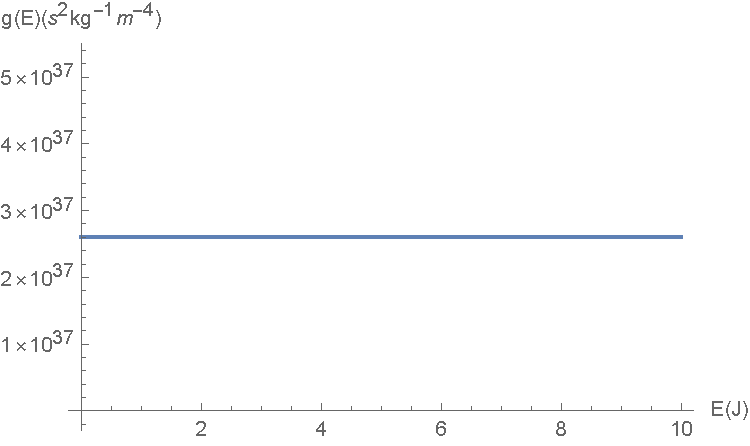
\includegraphics[width=0.5\linewidth]{density}
	      	\caption{2D DOS}
	      	\label{fig:density}
	      \end{figure}
	      The DOS is $g(E) = \frac{m}{\hbar^2\pi}$.
	\item
	      Now $L = 2l$,
	      so Fermi energy of $x-y$ plane will be\footnote{Note that here $N\neq \num{2.403e11}$.}
	      \begin{equation}
	      	E_{F} =  \frac{\hbar^2}{2m} 2\pi\frac{N}{L^2} = N\times \SI{3.84013e-30}{\joule},
	      \end{equation}
	      and $n$th energy level will be
	      \begin{equation}
	      	E_n = n^2\frac{\hbar^2\pi^2}{2m L^2} = n^2\times  \SI{8.97095e-20}{\joule}.
	      \end{equation}
	      When $n=1$, to make them equal,
	      there need to be $N_1 = \num{2.3361e10}$ electrons, i.e.~, this number of electrons are filled in the first
	      level of $z$ direction, after that, the rest electrons will simultaneously fill in both higher levels of
	      $z$ direction and the first level of $z$ direction (since it is not fully filled).
	      The Fermi energy of the second level is
	      \begin{equation}
	      	\begin{split}
	      		E_{F,2} &=  \frac{\hbar^2}{2m} 2\pi\frac{N_2}{L^2} - (\Delta E_2 - \Delta E_1)\\
	      		&= \num{3.84013e-30}\times N_2 \,\si{\joule} - \SI{2.691e-19}{\joule}
	      	\end{split}
	      \end{equation}
	      When $E_{F,2} = E_3$, electrons will then fill in the third energy level,
	      \begin{equation}
	      	E_3 = 9 \frac{\hbar^2\pi^2}{2m L^2} = \SI{8.07386e-19}{\joule}.
	      \end{equation}
	      And at this time, we need $N_2 = \num{2.80325e11}$. Because the DOS of the first level and the second level are the same, so it also needs $N_1$ amounts of electrons in the first level,
	      because the DOS of a 2D system is a constant $\frac{m}{\hbar^2\pi}$, we have
	      \begin{equation}
	      	N_1 = \frac{m}{\hbar^2\pi} \pi k_1^2,
	      \end{equation}
	      So the rest of electrons, which $N_3= N - N_1 -N_2$ are filled in the third level.
\end{enumerate}





\section*{Problem \RMN{4}}

The number of electrons are excited is of order $g(\varepsilon_F)k_B T$, their energy is of order $k_B T$.
So the total energy is
\begin{equation}
	E = E_0 + g(\varepsilon_F) (k_B T)^2.
\end{equation}
There is a coefficient difference $\frac{\pi^2}{6}$.
So the heat capacity is $\dfrac{\partial E}{\partial T} =2 g(\varepsilon_F) k_B^2 T$.










\bibliographystyle{unsrt}
\bibliography{ref}
\end{document}
